\documentclass{beamer}

\mode<presentation>
{
  \usetheme{Darmstadt}     
  \usecolortheme{default} 
  \usefonttheme{structurebold}
  \setbeamertemplate{navigation symbols}{}
  \setbeamertemplate{caption}[numbered]
} 

\usepackage[english]{babel}
\usepackage[utf8x]{inputenc}
\usepackage{xcolor}
\usepackage{listings}
\usepackage{multicol}
\lstset
{
    language=[LaTeX]TeX,
    breaklines=true,
    basicstyle=\tt\scriptsize,
    %commentstyle=\color{green}
    keywordstyle=\color{blue},
    %stringstyle=\color{black}
    identifierstyle=\color{magenta},
}

\title[Linear and Deformable Image Registration with 3D CNN]{Linear and Deformable Image Registration with 3D Convolutional Neural Networks}
\author{Stergios C. et al.}
\institute[MICCAI 2018]{Stoyanov D. et al. (eds) Image Analysis for Moving Organ, Breast, and Thoracic Images. RAMBO 2018, BIA 2018, TIA 2018 }
\date{Presented by - Kumar Shreshtha\\BITS Pilani}


\AtBeginSection[]
{
  \begin{frame}<beamer>
    \frametitle{Outline}
    \tableofcontents[currentsection,currentsubsection]
  \end{frame}
}

\begin{document}

\begin{frame}
  \titlepage
\end{frame}


\begin{frame}{Outline}
  \tableofcontents
\end{frame}

\section{Introduction}

\begin{frame}{Image Registration}
	\begin{itemize}
	    \item The process of establishing spatial correspondence between a source image $(I_S)$ and a target image $(I_T)$ to align them to the same coordinate system.
  		\pause
  		\item Optimization Problem:
		 \begin{block}{}
			\begin{center}$\theta^* = \underset{\theta}{min} C(I_T,T_{\theta}(I_S))$
			\end{center}
		\end{block}
                \begin{tabular}{l l l }
                    where&$C$ & cost function \\
                    &$I_T$ & target image \\
                    &$I_S$ & source image \\
                    &$\theta$ & transformation parameters\\
                    &$T_{\theta}$ & transformation function \\
                \end{tabular}
		\pause
		\item The task is to optimize a cost function over two images by tuning the parameters of a transformation function which tries to warp the source image to target image.
  	\end{itemize}
\end{frame}



\begin{frame}{Registration: Rigid vs Deformable}
	\begin{itemize}
  		\item Rigid/Linear Registration:
  		    \begin{itemize}
  		        \item Uses a simple transform, uniformly applied.
  		        \pause
  		        \item Rotations, translations, etc.
  		    \end{itemize}
  		\pause
  		\item Non-Rigid/Deformable Registration:
  		    \begin{itemize}
  		        \item Allows a non-uniform mapping between images.
  		        \pause
  		        \item Measure and/or correct small, varying discrepancies by deforming one image to match the other.
  		        \pause
  		        \item Vector field/deformation field $T_{\theta}$ is computed from $I_T$ to $I_S$.
  		        \item Inverse warp transform $I_S$ into $I_T$'s coordinate system.
  		    \end{itemize}
	\end{itemize}
\end{frame}

\begin{frame}{Deformable Registration: Clinical Relevance}
	\begin{itemize}
  		\item internal organs are non-rigid
  		\item physical brain deformations during neurosurgery
  		\item normal squishing, shifting and emptying of abdominal/pelvic organs and soft tissues
  		\item Patient motion during image scanning
  		\item \textbf{Lung motion during respiration}
	\end{itemize}
\end{frame}

\begin{frame}{Registration: ill-posed problem}
	\begin{itemize}
  		\item Well-posed problems:
  		\begin{itemize}
  		    \item solution exists
  		    \item is unique
  		    \item depends continuously on the data
  		\end{itemize}
  		\pause
  		\item Ambiguity between homogeneous regions. Multiple solutions possible.(not Unique)
  		\pause
  		\item Solution search space is often $\infty$-dimensional.
	\end{itemize}
\end{frame}

\begin{frame}{Registration: Cost Function}
    \begin{itemize}
        \item The cost/energy function typically comprises of two components:
        \pause
        \begin{block}{}
			\begin{center}$C(I_T,T_{\theta}(I_S)) = \mathcal{M}(I_T,I_S \circ T_{\theta})+\mathcal{R}(T_{\theta})$
			\end{center}
		\end{block}
		\begin{tabular}{l l l }
            where&$\mathcal{M}$ & quantifies level of alignment between $I_T$ and $I_S$\\ &$\mathcal{R}$& regularizes the transformation \\
        \end{tabular}
        \pause
        \item $\mathcal{R}$ aims to favor specific properties desired in the solution.
        \pause
        \item Helps tackle the ill-posedness of registration problem.
        \pause
        \item Adding a regularization term can provide \textbf{provable uniqueness} and a \textbf{computable subspace}.
    \end{itemize}
\end{frame}

\begin{frame}{Registration: Ingredients}
	\begin{itemize}
  		\item Image Registration Algorithm involves three main components:
  		    \begin{itemize}
  		        \pause
  		        \item deformation model - $T_{\theta}$
  		        \pause
  		        \item objective function - $C(I_T,T_{\theta}(I_S))$
  		        \pause
  		        \item optimization method
  		    \end{itemize}
  		\pause
  		\item The dependency of the registration result on the optimization strategy follows from the fact that image registration is inherently ill-posed.
  		\pause
  		\item Devising each component so that the requirements of the registration algorithm are met is a demanding process.
  		\pause
  		\item Modeling Complex Equations?
  		\pause
  		\item \textbf{Neural Networks!}
	\end{itemize}
\end{frame}


\begin{frame}{Existing Methods}
	\begin{itemize}
  		\item Drawbacks of state-of-the-art methods:
  		    \begin{itemize}
  		        \item Existing methods are often biased towards the linear component
  		        \item Sensitive to application setting
  		        \item involve multiple hyper-parameters
  		        \item computationally expensive
  		    \end{itemize}
  		\pause
  		\item Limitations of Deep learning based methods:
  		    \begin{itemize}
  		        \item dependency on linear component of the transformation
  		        \item \textbf{dependency on ground truth displacement (supervised learning)}
  		    \end{itemize}
	\end{itemize}
\end{frame}

\begin{frame}{Contributions of Stergios C. et al.}
	\begin{itemize}
  		\item coupling linear and deformable registration within a single architecture.
  		\item independent of different similarity metrics
  		\item reduced computational time
  		\item associating with clinical data to classify patients with interstitial lung disease (ILD).
	\end{itemize}
\end{frame}

\section{Methodology}

\begin{frame}{Dataset}
    \begin{itemize}
        \item MRI exams of 41 patients were acquired(29 with systemic sclerosis and 12 healthy)
        \item Lung fields were annotated for 82 images and were labeled as healthy/not healthy.
        \pause
        \item Pre-processing:
        \begin{itemize}
            \item image intensity values clipped between the range [0,1300] and normalized to [0,1].
            \item images were scaled down by a factor of 2/3 using cubic interpolation to a final size of 64x192x192.
            \item 28 patients data were selected for training using random sampling and remaining 13 were used for validation.
        \end{itemize}
    \end{itemize}
\end{frame}

\begin{frame}{Network Architecture}
    \begin{figure}
        \centering
        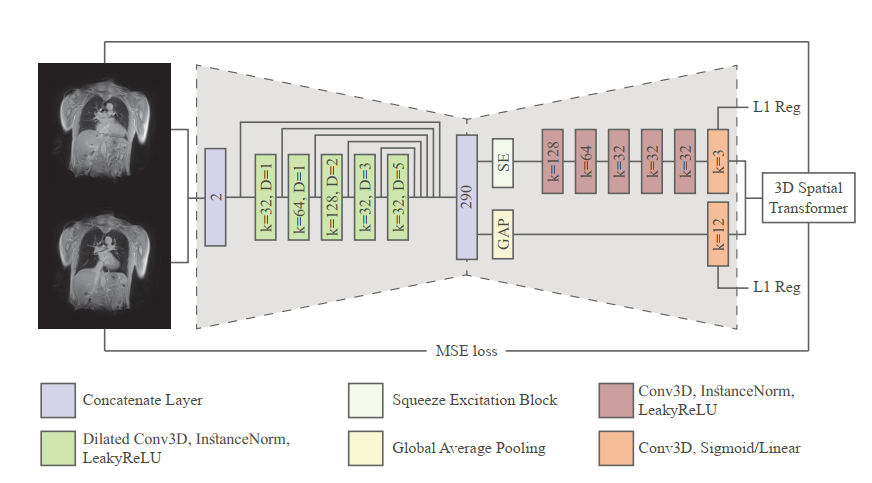
\includegraphics[height=6cm]{network_architecture.png}
        \caption{Overview of Network Architecture}
        \label{fig:overview}
    \end{figure}
\end{frame}

\begin{frame}{Network Architecture: PyTorch}
    \begin{figure}
        \centering
        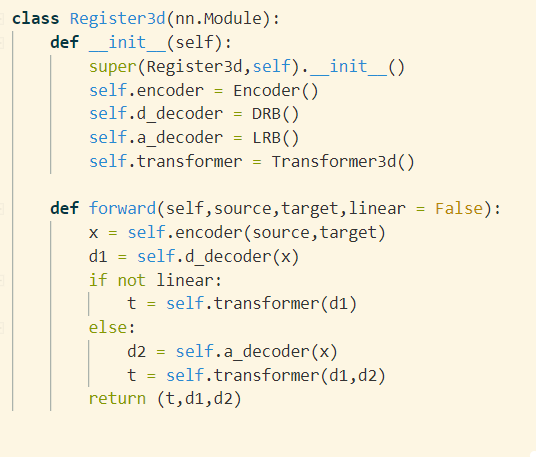
\includegraphics[height=6cm]{overview.PNG}
        \label{fig:code}
    \end{figure}
\end{frame}

\begin{frame}{Network Architecture: Encoder}
\begin{itemize}
    \item takes as input the source and target image concatenated along channels axis.
    \item Consists of 5 layers of 3x3x3 dilated convolutions each followed by instance normalization and LeakyReLU.
    \item the outputs of each layer are finally concatenated to provide multi-resolution feature merging which is then fed into the 2 branches of the decoder.
\end{itemize}
\end{frame}

\begin{frame}{Encoder: Insights}
    \begin{itemize}
    \item why dilated convolution?
    \begin{itemize}
        \item provides greater receptive field to compensate for no max-pooling.
        \item larger filters require more trainable parameters.
    \end{itemize}
    \pause
    \item gridding problem: as zeros are padded between two pixels in a convolutional kernel, the receptive field of this kernel only covers an area with checkerboard patterns - only locations with non-zero values are sampled, losing some neighboring information.
    \pause
    \item dilation rate increases as Fibonacci sequence (1,1,2,3,5) as opposed to exponentially. This mitigates the gridding problem by providing a less steep dilation rate increase and thus denser sampling.
\end{itemize}
\end{frame}

\begin{frame}{Encoder: Insights (Contd.)}
    \begin{itemize}
    \item Instance normalization
    \begin{itemize}
        \item provides invariance to intensity and contrast shift
        \item simplifies learning process
        \item could mitigate problems caused by difference in imaging devices.
    \end{itemize}
    \pause
    \item multi-resolution feature merging
    \begin{itemize}
        \item permits the aggregation of features from all different scales and levels of abstraction
        \item facilitates the flow of gradients through the network and therefore allows faster training.
    \end{itemize}
\end{itemize}
\end{frame}

\begin{frame}{Encoder: PyTorch}
    \begin{figure}
        \centering
        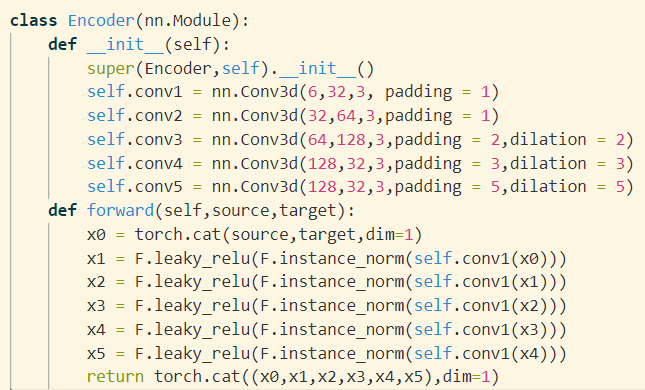
\includegraphics[height=6cm]{encoder.png}
        \label{fig:encoder}
    \end{figure}
\end{frame}

\begin{frame}{Network Architecture: Decoder}
\begin{itemize}
    \item comprises of two branches each of which produces a sampling grid 
        \begin{itemize}
            \item for Linear Registration
            \item for Deformable Registration
        \end{itemize}
        respectively.
    \pause
    \item \textbf{Linear Registration Branch (LRB)} comprises of a global average pooling layer followed by 1x1x1 3D convolutions with linear activation to produce 12(3x4) activation values which acts as the affine transformation matrix. This affine matrix is then used to compute a sampling grid for linear registration.
    \pause
    \item \textbf{Deformable Registration Branch (DRB)} comprises of a squeeze and excitation block followed by multiple 3x3x3 convolutions each followed by instance norm and LeakyReLU. The final layer has sigmoid activation and its activations are multiplied by 2 to get a spatial gradient sampling grid.
\end{itemize}
\end{frame}
\begin{frame}{Decoder: PyTorch}
    
    \begin{figure}
        \centering
        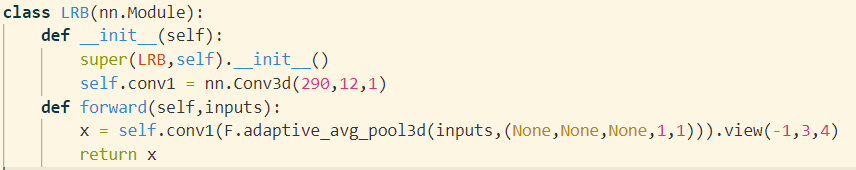
\includegraphics[height=2cm]{LRB.PNG}
        \label{fig:code_decoder}
    \end{figure}

    \begin{figure}
        \centering
        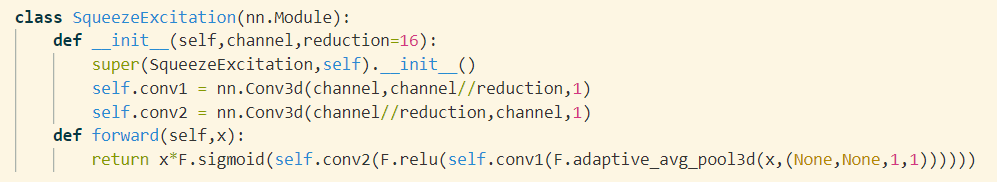
\includegraphics[height=2cm]{seblock.PNG}
        \label{fig:code_decoder_2}
    \end{figure}
    
\end{frame}

\begin{frame}{Decoder: PyTorch}

    \begin{figure}
        \centering
        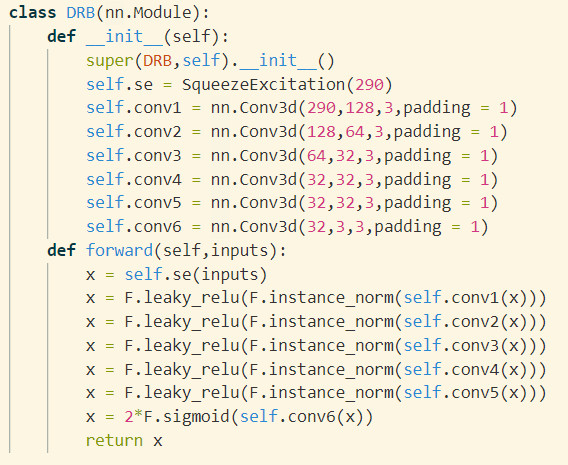
\includegraphics[height=6cm]{drb.PNG}
        \label{fig:code_decoder_3}
    \end{figure}
    
\end{frame}

\begin{frame}{Deformable Registration Branch (DRB) : Insights}
    \begin{columns}
		\begin{column}{4cm}
			\begin{figure}
  				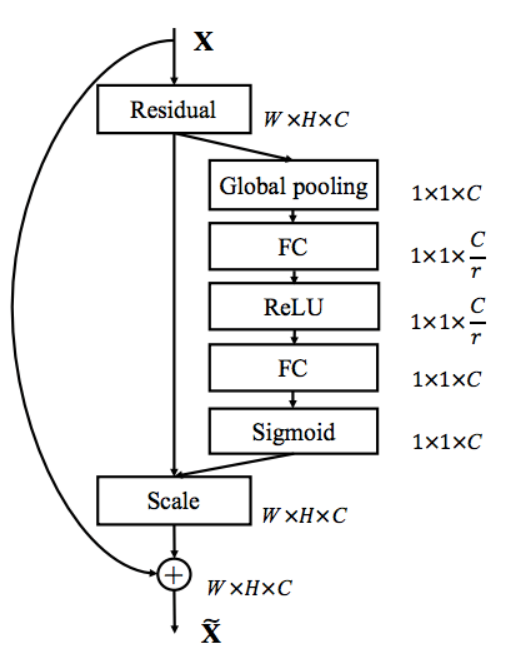
\includegraphics[height=6cm]{senet.png}
			\end{figure}
        \end{column}
        \begin{column}{6cm}
            \begin{itemize}
                \item Squeeze and Excitation Block:
                    \begin{itemize}
                        \item in a normal convolution operation all channels contribute equally to the output feature map.
                        \item SE-block allows to add an adaptive scale to control the contribution of each input channel to the output feature map.
                    \end{itemize}
            \end{itemize}
        \end{column}
    \end{columns}
    
\end{frame}

\begin{frame}{Deformable Registration Branch (DRB) : Insights}
    \begin{itemize}
        \item The final output of the DRB is a 3 channel 3d-feature map of same spatial dimensions as the target image with values in range [0,2].
        \pause
        \item Thus, for each voxel we have 3 values between [0,2] representing the spatial gradient along each of the three axes (x,y,z).
        \pause
        \item The spatial gradient gives a measure of displacement of consecutive pixels.
        \pause
        \item limiting the maximum value of gradients to two allows for control of maximum displacements among consecutive pixels. 
        \pause
        \item such an approach ensures generation of smooth deformations that avoid self-crossing.
    \end{itemize}
\end{frame}


\begin{frame}{Deformable Registration Branch (DRB) : Insights}
	\begin{figure}
  		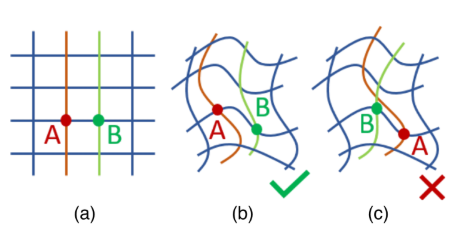
\includegraphics[height=5cm]{self-crossing.png}
	\end{figure}
    Non-negative values for spatial gradients ensure no \textbf{self-crossing}.
\end{frame}
\begin{frame}{Deformable Registration Branch (DRB) : Insights}
    \begin{itemize}
        \item A spatial gradient value of 1 indicates there is no change in the distance between the consecutive pixels along the given axis.
        \item A value less than 1 indicate the distance between the pixels will decrease along the given axis.
        \item  A value greater than 1 indicate the distance between the pixels will increase along the given axis.
    \end{itemize}
    \pause
    \begin{block}{Generating sampling grid from spatial gradients}
    \centering
    $[G(p)]_d = \sum_{i=0}^{p}\phi_{id}$
    \end{block}
    \begin{tabular}{l l l }
                    with&$[G(p)]_d$ & d-component of sampling grid G at voxel p  \\
                    &$\phi_{id}$ & d-component of spatial gradient $\phi$ at voxel i \\
    \end{tabular}
\end{frame}

\begin{frame}{Linear Registration Branch (LRB)}
    \begin{itemize}
        \item once the affine transformation matrix is calculated using the above procedure we can generate the sampling grid for each voxel in the deformed image using the following formula:
        \begin{block}{Generating sampling grid from affine matrix}
            \begin{center}
            $\begin{pmatrix} 
                {x}_{i}^s \\ 
                {y}_{i}^s\\ 
                {z}_{i}^s  
            \end{pmatrix}
            = 
            \begin{bmatrix} 
                \theta_{11} & \theta_{12} & \theta_{13} & \theta_{14}\\ 
                \theta_{21} & \theta_{22} & \theta_{23} & \theta_{24}\\
                \theta_{31} & \theta_{32} & \theta_{33} & \theta_{34} 
             \end{bmatrix}
            \begin{pmatrix} 
                {x}_{i}^t \\ 
                {y}_{i}^t\\ 
                {z}_{i}^t\\
                1
            \end{pmatrix}$
            \end{center}
        \end{block} 
    \end{itemize}
\end{frame}

\begin{frame}{3D Spatial Transformer}
    \begin{itemize}
        \item the 3D transformer layer takes as input the source(moving) image (S), the linear($G_A$) and deformable ($G_N$) sampling grids and  performs the sampling operation $\mathcal{W}$ to produce the deformed image D.
        \item first the deformable grid is applied and to its output the linear sampling grid is applied:
        \begin{block}{}
            \centering
            $\mathcal{W}(S,G) = \mathcal{W}(\mathcal{W}(S,G_N),G_A)$
        \end{block}
    \end{itemize}
    \begin{figure}
  		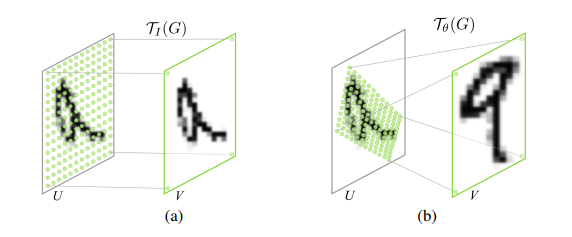
\includegraphics[height=3cm]{transformer.png}
	\end{figure}
\end{frame}

\begin{frame}{3D Spatial Transformer}
    \begin{itemize}
        \item The warping operation $(\mathcal{W})$ must be differentiable with respect to the input image (S) and the deformation(G) in order to allow back-propagation training.
        \pause
        \item The warping function is thus defined as a trilinear interpolation sampling as follows:
        \begin{block}{}
            \centering
            $\mathcal{W}(S,G)(\textbf{p}) = \underset{\textbf{q}}{\sum}S(\textbf{q})\underset{d}{\prod}max(0,1-|[G(\textbf{p})]_d-\textbf{q}_d|)$
        \end{block}
        %\pause
        % \item And hence the computed gradients for backprop are as follows:
        % \begin{block}{}
        %     \centering
        %     $\frac{\partial \mathcal{W}(S,G)}{\partial S(\textbf{q})} = \underset{\textbf{q}}{\sum}\underset{d}{\prod}max(0,1-|[G(\textbf{p})]_d-\textbf{q}_d|)$\\
        %     $\frac{\partial \mathcal{W}(S,G)}{\partial \textbf{q}_{d_i}} = \underset{\textbf{q}}{\sum}S(\textbf{q})\underset{D-\{d_i\}}{\prod}max(0,1-|[G(\textbf{p})]_d-\textbf{q}_d|)$
        % \end{block}
    \end{itemize}
\end{frame}

\begin{frame}{Training}
    
        \begin{block}{Loss Function}
        \begin{center}
        $Loss = || R - \mathcal{W}(S,G) ||^2 + \alpha||A-A_I||_1 + \beta||\Phi-\Phi_I||_1$
        \end{center}
    \end{block}
    \pause
    \begin{itemize}
        \item Why regularization?
        \begin{itemize}
            \pause
            \item Without L1 regularization on A high reconstruction error may occur as the network might get stuck in a local minimum where it aligns only high level features.
            \pause
            \item Without the smoothness regularizer on $\phi$, spatial gradients decoder network can predict very non-smooth grids which makes it prone to fall in local minimum.
        \end{itemize}
    \end{itemize}
    
    
\end{frame}

\begin{frame}{Training (Contd.)}
    hyper-parameters:
        \begin{itemize}
            \item \textbf{optimizer:} Adam 
            \item \textbf{initial learning rate:}$10^{-3}$
            \item \textbf{reduce LR on plateau:} 
                \begin{itemize}
                    \item patience: 50 epochs
                    \item factor: 0.9
                \end{itemize}
            \item \textbf{early stopping patience :} 100 epochs
            \item \textbf{batch size:} 2
            \item \textbf{regularizers:} $\alpha = \beta = 10^{-6}$
        \end{itemize}
\end{frame}

\section{Experiments}
\begin{frame}{Evaluation}
    \begin{itemize}
        \item Dice Coefficient Metric
        \begin{itemize}
            \item measured on lung masks after source deformation.
        \end{itemize}
        \item Average error over all axes of predicted locations for 11 manually annotated landmark points was also calculated.
        \item Compared with two different state-of-the-art methods
            \begin{itemize}
                \item Symmetric Normalization(SyN)
                \item deformable method with variety of similarity metrics (MI,NCC,DWM)
            \end{itemize}
    \end{itemize}
\end{frame}

\begin{frame}{Results}
    \begin{itemize}
        \item Two different types of test:
            \begin{itemize}
                \item Inhale-Exhale (13 validation pairs)
                \item All combinations (169 validation pairs)
            \end{itemize}
    \end{itemize}
    \begin{table}
    \centering
    \scriptsize
    \begin{tabular}{l r r r}
        \hline Method & Inhale-Exhale & All Combinations & Time/subject(s)\\\hline
         Unregistered & 75.620$\pm$10.89 & 57.22$\pm$12.90 & -\\
         Deformable with NCC & 84.25$\pm$6.89 & 76.10$\pm$7.92 & ~1(GPU)\\
         Deformable with DWM & 88.63$\pm$4.67 & 75.92$\pm$8.81 & ~2(GPU)\\
         Deformable with MI & 88.86$\pm$5.13 & 76.33$\pm$8.74 & ~2(GPU)\\
         Deformable with all above & 88.81$\pm$5.85 & 78.71$\pm$8.56 & ~2(GPU)\\
         SyN & 83.86$\pm$6.04 & - & ~2500(CPU)\\
         Proposed w/o Affine & 91.28$\pm$2.47 & 81.75$\pm$7.88 & ~0.5(GPU)\\
         Proposed & \textbf{91.48$\pm$2.33} & \textbf{82.34$\pm$7.68} & ~0.5(GPU)\\\hline
    \end{tabular}
    \caption{Dice Coefficient Score(\%) calculated over the deformed lung masks and the ground truth}
    \label{performance_table}
    \end{table}
\end{frame}

\begin{frame}{Results (Contd.)}
    \begin{table}
    \centering
    \small
    \begin{tabular}{l l l l l}
        \hline Method & dx & dy & dz & ds\\\hline
         Inter-observer & 1.664 & 2.545 & 1.555 & 3.905\\
         Deformable with NCC,DWM and MI  & 1.855 & 3.169 & 2.229 & 4.699\\
         Proposed w/o Affine  & 2.014 & 2.947 & 1.858 & 4.569\\
         Proposed  & 1.793 & 2.904 & 1.822 & 4.358\\\hline
    \end{tabular}
    \caption{Errors measured as average euclidian distances between estimated landmark locations and ground truth marked by two medical experts.}
    \label{comparision_table}
    \end{table}
\end{frame}

\begin{frame}{Results: Analysis}
    Majority of the errors occur at boundaries, indicating that large local displacements are not captured
    \begin{figure}
        \centering
        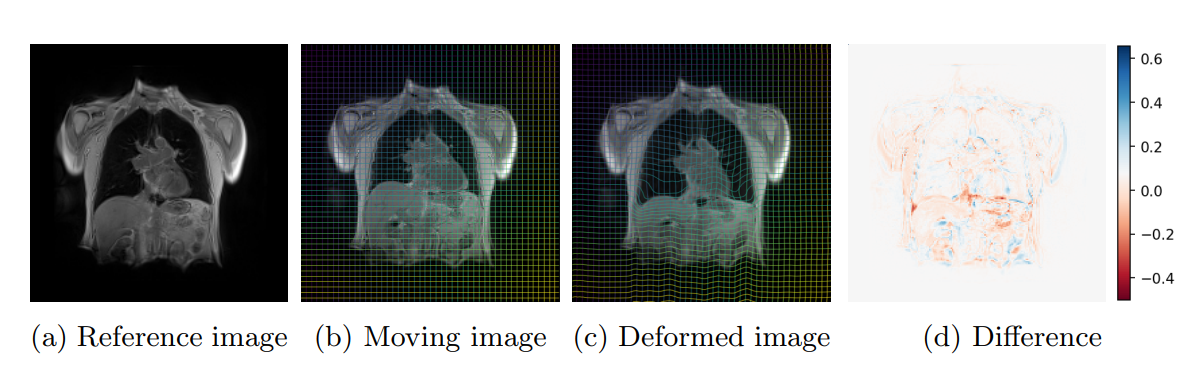
\includegraphics[height=3.5cm]{results.png}
        \caption{Registration generated by the proposed architecture}
        \label{fig:results}
    \end{figure}
\end{frame}

\begin{frame}{Evaluation of Clinical Relevance}
    \begin{itemize}
        \item a small classifier is trained for assessing clinical relevance.
        \item residual deformation $(G_{\delta}=G-G_I)$ indicating voxel displacement is fed as input to a shallow neural network which classifies patients as healthy/unhealthy.
        \item binary crossentropy was used as loss function and initial learning rate $10^{-4}$, which was halved every 50 epochs.
        \item 5 models were trained in parallel for 5-fold cross validation and an accuracy of 84.62 \% is reported.
    \end{itemize}
\end{frame}

\begin{frame}{Evaluation of Clinical Relevance: Model}
    \begin{figure}
        \centering
        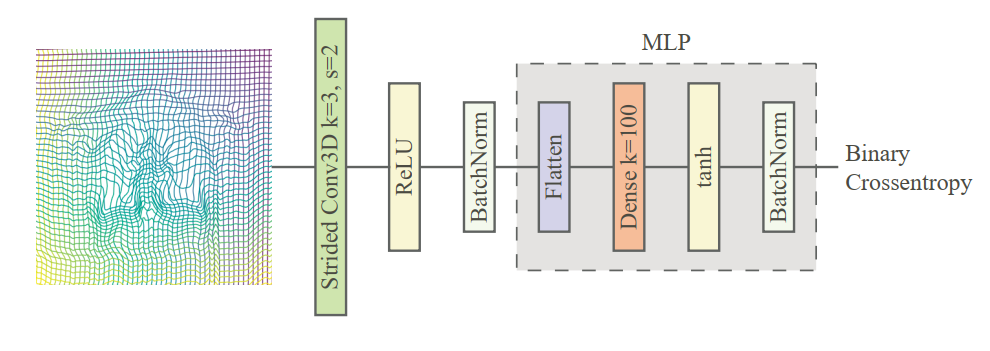
\includegraphics[height=4cm]{MLP.png}
        \caption{ILD Classifier}
        \label{fig:MLP}
    \end{figure}
\end{frame}

\section{Conclusion}
	
\begin{frame}{Conclusion}
    \begin{itemize}
        \item The paper presents an unsupervised end-to-end deep learning model for image registration using an optimal transformation between pair of images.
        \item the model is modular with respect to similarity functions and nature of transformation
        \item promising results compared to other unsupervised methods
        \item generates deformations with no self-crossings
        \item computationally efficient due to GPU implementation 
        \item \textbf{Future Scope:} Evaluation of the proposed model on registration of other modalities and other organs.
    \end{itemize}
	
\end{frame}
\end{document}
